\documentclass[12pt,a4paper]{article}

\usepackage[romanian]{babel}
\usepackage[T1]{fontenc}
\usepackage[utf8]{inputenc}
\usepackage{lmodern}
\usepackage{listings}
\usepackage{xcolor}
\usepackage{hyperref}
\usepackage{geometry}
\usepackage{mdframed}
\usepackage{amsmath}
\usepackage{amssymb}
\usepackage{tikz}
\usepackage{graphicx}
\usepackage{float}

\usetikzlibrary{shapes.geometric, arrows.meta}

\geometry{margin=2.5cm}

\lstset{
  basicstyle=\ttfamily\small,
  backgroundcolor=\color{gray!10},
  frame=single,
  breaklines=true,
  showstringspaces=false,
  language=C,
  literate=
    {ă}{{\u{a}}}1
    {â}{{\^{a}}}1
    {î}{{\^{\i}}}1
    {ș}{{\c{s}}}1
    {ț}{{\c{t}}}1
    {Ă}{{\u{A}}}1
    {Â}{{\^{A}}}1
    {Î}{{\^{I}}}1
    {Ș}{{\c{S}}}1
    {Ț}{{\c{T}}}1,
}

\lstdefinestyle{shell}{
  language=bash,
  basicstyle=\ttfamily\small,
  backgroundcolor=\color{gray!10},
  frame=single,
  breaklines=true,
  showstringspaces=false,
}

\title{Laboratorul 4 \\ Procese}
\date{}

\begin{document}

\maketitle

\vspace{-40pt}

\section{Ce este un proces?}

Un sistem de operare execută o varietate de \textit{programe} 
care rulează ca și \textit{procese}.

\begin{center}
  \begin{minipage}{0.45\textwidth}
    \begin{mdframed}[linecolor=gray, linewidth=0.5pt, backgroundcolor=gray!7,
      innertopmargin=8pt, innerbottommargin=8pt]
      \centering
      \textbf{Program} \\[6pt]
      \raggedright
      Un fișier executabil static, cu instrucțiuni și date, 
      stocat pe disk, care nu face nimic până nu este lansat în execuție.
    \end{mdframed}
  \end{minipage}
  \hfill
  \begin{minipage}{0.45\textwidth}
    \begin{mdframed}[linecolor=gray, linewidth=0.5pt, backgroundcolor=gray!7,
      innertopmargin=8pt, innerbottommargin=8pt]
      \centering
      \textbf{Proces} \\[6pt]
      \raggedright
      Un program aflat în execuție, cu o stare proprie în memorie, resurse
      alocate și un context de execuție activ.
    \end{mdframed}
  \end{minipage}
\end{center}

$\rightarrow$ Un program devine proces atunci cand 
un fișier executabil este încărcat în memorie.

\medskip
\textbf{Analogie:} \textit{programul} este rețeta, 
\textit{procesul} este gătitul $\rightarrow$ 
același program poate genera mai multe procese simultan, 
fiecare independent de celelalte.
\medskip

Informațiile despre procese sunt ținute într-o structură numită 
\texttt{Process Control Block (PCB)}, numită și \texttt{task control block},
câte una pentru fiecare process existent în sistem. 
Printre cele mai importante informații 
conținute de \texttt{PCB} regăsim:

\begin{center}
  \begin{minipage}{0.70\textwidth}
    \begin{itemize}
      \setlength{\itemsep}{0.75pt}
      \item \texttt{PID} (process ID);
      \item \texttt{PPID} (parent process ID); 
      \item spațiul de adrese;
      \item starea procesului -- running, waiting, etc;
      \item registre generale, \texttt{PC} (contor program), \\
      \texttt{SP} (indicator stivă);
      \item tabela de fișiere deschise;
      \item informații referitoare la semnale;
      \item informații referitoare la sistemele de fișiere \\
      (directorul rădăcină).
    \end{itemize}
  \end{minipage}
  \hfill
  \begin{minipage}{0.26\textwidth}
    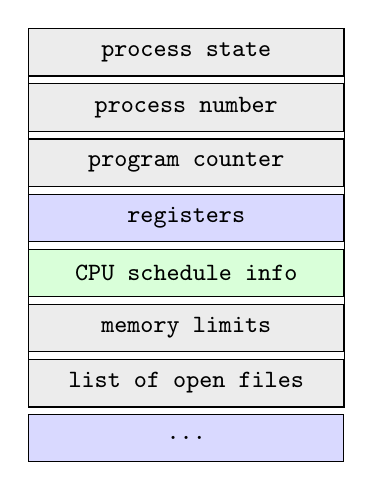
\begin{tikzpicture}
      \tikzstyle{block} = [draw, rectangle, minimum width=4cm,
                           minimum height=0.6cm, align=center,
                           font=\small\ttfamily]
      \tikzstyle{blockblue} = [block, fill=blue!15]
      \tikzstyle{blockgray} = [block, fill=gray!15]
      \tikzstyle{blockgreen} = [block, fill=green!15]

      \node[blockgray] (s1) at (0,0)    {process state};
      \node[blockgray] (s2) at (0,-0.7) {process number};
      \node[blockgray] (s3) at (0,-1.4) {program counter};
      \node[blockblue] (s4) at (0,-2.1) {registers};
      \node[blockgreen] (s5) at (0,-2.8) {CPU schedule info};
      \node[blockgray] (s6) at (0,-3.5) {memory limits};
      \node[blockgray] (s7) at (0,-4.2) {list of open files};
      \node[blockblue] (s8) at (0,-4.9) {\ldots};

      \draw (s1.north west) rectangle (s7.south east);
    \end{tikzpicture}
  \end{minipage}
\end{center}

\medskip
\textbf{Spațiul de adrese} al unui proces este izolat de cel al celorlalte procese 
și se împarte în mai multe zone:
\begin{itemize}
  \setlength{\itemsep}{0.75pt}
  \item \textbf{Zona de cod} (\textit{text section}) -- instrucțiunile programului;
  \item \textbf{Zona de date} (\textit{data section}) -- variabilele globale și statice;
  \item \textbf{Heap-ul} -- memorie alocată dinamic (ex. malloc);
  \item \textbf{Stiva} (\textit{stack}) -- date temporare precum: parametrii funcțiilor,
  adrese de return, variabile locale.
\end{itemize}
\medskip

\vspace{-50pt}

\begin{figure}[H]
  \centering
  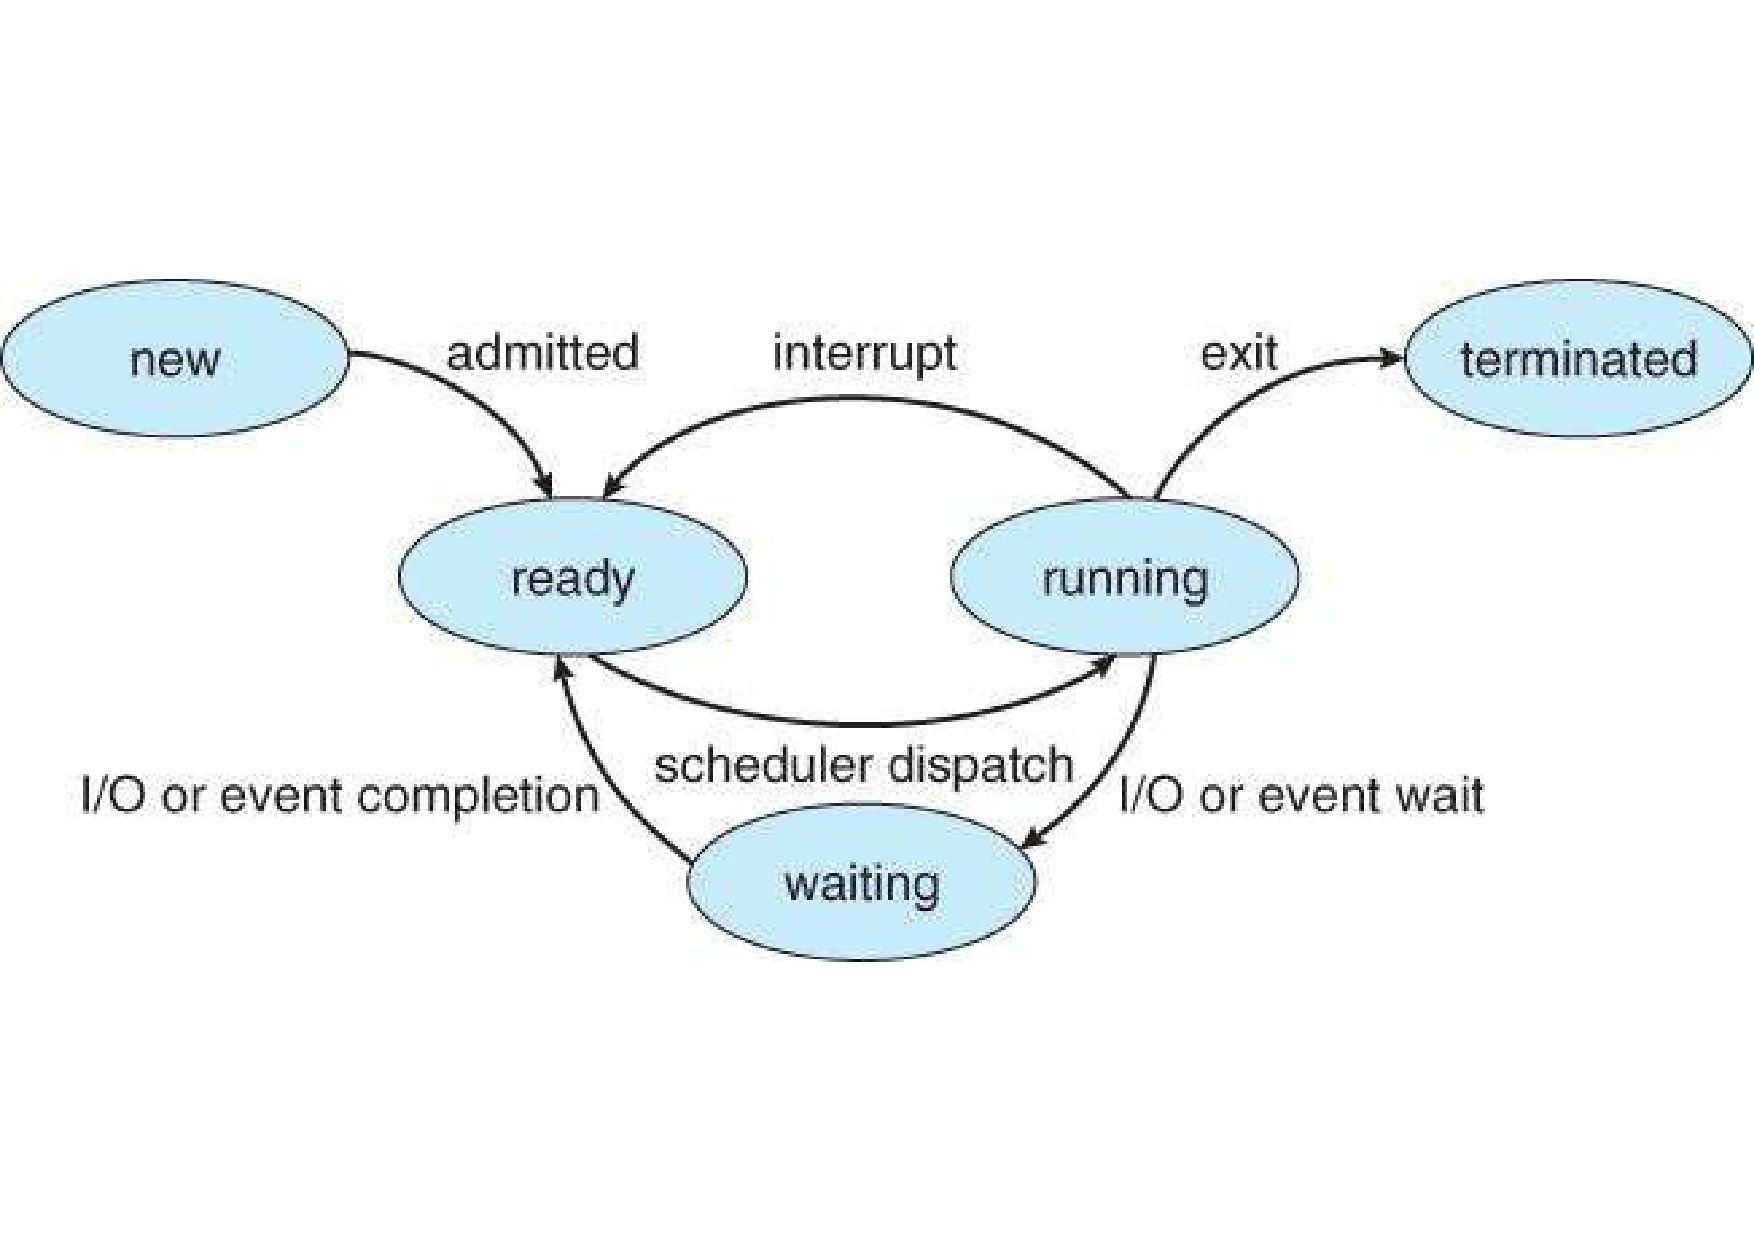
\includegraphics[width=0.8\textwidth]{ProcessState.pdf}
  \vspace{-60pt}
  \caption{Diagrama stărilor unui proces.}
  \label{fig:process-state}
\end{figure}
\vspace{-10pt}
{\scriptsize \textit{Sursă: Abraham Silberschatz, Peter B. Galvin, Greg Gagne,
``Operating System Concepts'', 10th Edition.}}

\medskip
\textbf{Stările unui proces}
\begin{itemize}
  \setlength{\itemsep}{0.75pt}
  \item \textbf{New}: procesul este inițiat;
  \item \textbf{Running}: procesul rulează;
  \item \textbf{Waiting}: procesul așteaptă un eveniment;
  \item \textbf{Ready}: procesul așteaptă să fie alocat unui procesor;
  \item \textbf{Terminated}: procesul și-a terminat execuția.
\end{itemize}
\medskip

\vspace{-20pt}
\begin{mdframed}[linecolor=gray, linewidth=0.5pt, backgroundcolor=gray!7,
  innertopmargin=6pt, innerbottommargin=6pt]
  \textbf{Starea zombie.} Un proces terminat care nu a fost încă \textit{recoltat}
  de părintele său (prin \texttt{wait(2)}) rămâne în sistem ca proces
  \textit{zombie} -- nu mai execută nimic, dar ocupă o intrare în tabela de procese
  până când părintele îi citește codul de retur. De aceea este important ca orice
  proces părinte să apeleze \texttt{wait(2)} după ce creează copii.
\end{mdframed}

\textbf{Scheduler-ul} este componenta din cadrul \textit{kernelului} 
care se ocupă de gestionarea proceselor. 
Acesta selectează procesele și le atribuie 
unuia dintre \textit{core-urile} procesorului 
pentru a fi rulate în funcție de prioritate, 
bazându-se pe o serie de algoritmi. \\

\textbf{Sistemul de fișiere \texttt{/proc}} \\
\indent Linux expune informații despre procesele active 
printr-un sistem de fișiere virtual numit \texttt{/proc}. 
Acesta nu există pe disk, ci este generat de kernel în timp real 
și conține câte un director pentru fiecare proces activ, 
denumit după PID-ul său.

\begin{lstlisting}[style=shell]
$ ls /proc/
1/   1234/   123456/   cpuinfo   meminfo   sys/   tty/   ...
\end{lstlisting}

În interiorul directorului unui proces se găsesc fișiere care expun informațiile
din task control block-ul acestuia:

\begin{itemize}
  \setlength{\itemsep}{0.75pt}
  \item \texttt{cmdline} -- comanda cu care a fost lansat procesul;
  \item \texttt{status} -- stare, PID, PPID, utilizator, memorie utilizată;
  \item \texttt{fd/} -- directorul cu fișierele deschise ale procesului;
  \item \texttt{maps} -- harta spațiului de adrese (cod, date, heap, stivă);
  \item \texttt{cwd} -- symlink către directorul curent al procesului.
\end{itemize}

Puteți inspecta procesul curent al shell-ului folosind variabila specială
\texttt{\$\$}, care conține PID-ul shell-ului activ:

\begin{lstlisting}[style=shell]
$ ls /proc/$$
$ cat /proc/$$/status
$ ls -la /proc/$$/fd
\end{lstlisting}

\begin{mdframed}[linecolor=gray, linewidth=0.5pt, backgroundcolor=gray!7,
  innertopmargin=6pt, innerbottommargin=6pt]
  \textbf{Bonus:} Nu toate sistemele de operare pot rula mai multe procese
  simultan. Sistemele \textbf{monotasking} (ex. MS-DOS) rulează doar un singur
  proces la un moment dat. Sistemele \textbf{multitasking} (ex. UNIX, Linux,
  Windows) pot rula mai multe procese simultan, pe procesoare diferite sau 
  alternat pe același procesor, creând iluzia execuției paralele.
\end{mdframed}

\section{Crearea unui proces nou}

În mediile de dezvoltare UNIX, funcția sistem cu care se creează 
procese noi este \texttt{fork(2)}. 
Odată invocată, funcția creează un proces nou 
(numit \textit{proces copil}),
acesta fiind o copie a procesului apelant, 
dar cu câteva diferențe, dintre care le enumerăm aici 
pe cele mai importante 
(ele pot diferi de la sistem de operare la sistem de operare):

\begin{itemize}
  \setlength{\itemsep}{0.75pt}
  \item procesul copil are ca părinte chiar pe 
  procesul ce a apelat \texttt{fork(2)}
  (în vreme ce procesul apelant va avea un alt părinte);
  \item procesul copil are un ID (denumit și \texttt{pid}) 
  diferit de cel al părintelui;
  \item procesul copil are un singur fir de execuție 
  (\textit{thread}, v. Laboratorul 6);
  \item procesul copil pornește de la zero în ceea ce privește 
  resursele utilizate și timpul de execuție, 
  precum și alți indicatori similari de gestionare a proceselor.
\end{itemize}

Din momentul apelului, dacă acesta este încheiat cu succes, 
fiecare viitoare instrucțiune va fi executată atât de părinte, 
cât și de copil. 
Diferențierea se face în funcție de
valoarea de retur a lui \texttt{fork(2)}: 
copilul primește valoarea \texttt{0} iar părintele
pid-ul copilului. 
Astfel, o construcție tipică C este:

\begin{lstlisting}
pid_t pid = fork();
if (pid < 0)
    return errno;
else if (pid == 0)
    /* child instructions */
else
    /* parent instructions */
\end{lstlisting}

Oricând în timpul execuției putem afla pid-ul procesului curent 
și pe cel al procesului părinte 
cu ajutorul funcțiilor \texttt{getpid(2)} și, respectiv, \texttt{getppid(2)}.

\begin{lstlisting}
printf("Parent %d Me %d\n", getppid(), getpid());
\end{lstlisting}

Părintele își poate suspenda activitatea 
pentru a aștepta finalizarea execuției unui proces copil 
cu ajutorul funcției \texttt{wait(2)}, 
care oferă ca valoare de retur pid-ul copilului.

Operația este utilă pentru a sincroniza și ordona instrucțiunile:

\begin{lstlisting}
pid_t pid = fork();
if (pid < 0)
    return errno;
else if (pid == 0) {
    /* child instructions */
    printf("First!");
} else {
    /* parent instructions */
    wait(NULL);
    printf("Last!");
}
\end{lstlisting}

\begin{mdframed}[linecolor=gray, linewidth=0.5pt, backgroundcolor=gray!7,
  innertopmargin=6pt, innerbottommargin=6pt]
  \textbf{Atenție:} Funcția \texttt{wait(2)} redă control părintelui 
  când se termină execuția \textit{oricăruia} dintre copiii săi. 
  Pentru cazuri complexe, în care se dorește 
  așteptarea unuia sau mai multor procese anume, 
  se pot folosi funcții avansate precum 
  \texttt{waitpid(2)} sau \texttt{wait4(2)}, 
  dar care nu fac obiectul laboratorului.
\end{mdframed}

\section{Executarea unui program existent}

Executarea unui program se realizează cu ajutorul apelului sistem \texttt{execve(2)}.

\begin{lstlisting}
int execve(const char *path, char *const argv[], char *const envp[]);
\end{lstlisting}

Aceasta suprascrie complet procesul apelant cu un nou proces, 
conform programului găsit la calea indicată în \texttt{path}.

\begin{mdframed}[linecolor=gray, linewidth=0.5pt, backgroundcolor=gray!7,
  innertopmargin=6pt, innerbottommargin=6pt]
  \textbf{Atenție:} Calea trebuie să fie absolută, 
  de exemplu \texttt{/bin/pwd} și nu \texttt{pwd}. 
  Pentru a obține această cale, puteți folosi comanda \texttt{which(1)}:
  \begin{lstlisting}[style=shell]
$ which pwd
/bin/pwd
$ which vi
/usr/bin/vi
  \end{lstlisting}
\end{mdframed}

Argumentele programului sunt puse în \texttt{argv} 
respectând convenția obișnuită din C:
pe prima poziție (\texttt{argv[0]}) se află calea absolută 
către program urmată de argumente.
Lista se încheie cu \texttt{null}. 
Variabilele de sistem din mediul de execuție sunt puse în
ultimul argument \texttt{envp}. 
Aceasta este o listă de șiruri de caractere similară cu
\texttt{argv} exceptând convenția primului element.

Din cauza efectului distructiv asupra procesului curent, 
\texttt{execve(2)} este adesea folosit împreună cu 
\texttt{fork(2)} astfel încât procesul nou-creat să fie cel suprascris.

\newpage

\begin{lstlisting}
pid_t pid = fork();
if (pid < 0)
    return errno;
else if (pid == 0) {
    /* child instructions */
    char *argv[] = {"pwd", NULL};
    execve("/bin/pwd", argv, NULL);
    perror(NULL);
} else
    /* parent instructions */
\end{lstlisting}

Având în vedere suprascrierea procesului curent, 
\texttt{execve(2)} nu mai revine în programul inițial 
decât în cazul în care a apărut o eroare, 
folosindu-se \texttt{errno} pentru a determina cauza. 
Cele mai des întâlnite erori sunt calea greșită sau lipsa lui
\texttt{argv}.

\section{Sarcini de laborator}

\begin{enumerate}

  \item Creați un proces nou folosind \texttt{fork(2)} 
  și afișați fișierele din directorul curent cu ajutorul \texttt{execve(2)}. 
  Din procesul inițial afișați pid-ul propriu și pid-ul copilului. 
  De exemplu:
\begin{lstlisting}[style=shell]
$ ./forkls
My PID=41875, Child PID=62668
Makefile  collatz.c  forkls.c  so-lab-4.tex
collatz   forkls     ncollatz.c
Child 62668 finished
\end{lstlisting}

  \item Ipoteza Collatz spune că plecând de la orice număr natural, 
  dacă aplicăm repetat următoarea operație:
    \[
      n \mapsto
      \begin{cases}
        n/2 & \text{dacă } n \equiv 0 \pmod{2} \\
        3n + 1 & \text{dacă } n \not\equiv 0 \pmod{2}
      \end{cases}
    \]
    șirul ce rezultă va atinge valoarea 1. 
    Implementați un program care folosește \texttt{fork(2)} 
    și testează ipoteza generând șirul asociat unui număr dat în procesul
    copil. \\

    Exemplu:
\begin{lstlisting}[style=shell]
$ ./collatz 24
24: 24 12 6 3 10 5 16 8 4 2 1.
Child 52923 finished
\end{lstlisting}

  \item Implementați un program care să testeze ipoteza Collatz 
  pentru mai multe numere date. 
  Pornind de la un singur proces părinte, 
  este creat câte un copil care se ocupă de un singur număr. 
  Părintele va aștepta să termine execuția fiecare copil. 
  Programul va demonstra acest comportament folosind funcțiile 
  \texttt{getpid(2)} și \texttt{getppid(2)}. 
  Exemplu:
\begin{lstlisting}[style=shell]
$ ./ncollatz 9 16 25 36
Starting parent 6202
9: 9 28 14 7 22 11 34 17 52 26 13 40 20 10 5 16 8 4 2 1.
36: 36 18 9 28 14 7 22 11 34 17 52 26 13 40 20 10 5 16 8 4 2 1.
Done Parent 6202 Me 40018
Done Parent 6202 Me 30735
16: 16 8 4 2 1.
25: 25 76 38 19 58 29 88 44 22 11 34 17 52 26 13 40 20 10 5 16 8 4 2 1.
Done Parent 6202 Me 13388
Done Parent 6202 Me 98514
Done Parent 58543 Me 6202
\end{lstlisting}

\end{enumerate}

\end{document}
